\documentclass{article}

\usepackage[utf8]{inputenc}
\usepackage{graphicx}
\usepackage{listings}
\lstset{language=C++}
\usepackage{hyperref}
\usepackage{amsthm}
\usepackage{amsfonts}
\usepackage{lscape}
\usepackage{multirow}

\theoremstyle{remark}
\newtheorem{tutorial}{Tutorial }

\title{{\tt vle.discrete-time} : simulation of 
discrete time models into VLE.}

%%%%%%%%%%%%
\begin{document}

\maketitle

\tableofcontents

%%%%%%%%%%%%
\section{Introduction}

The first objective of this work is to improve the current extension \\
 {\tt vle.extension.difference-equation} for modeling recurrent relations.
 The second objective is to go further by providing a base extension for all
discrete time atomic models.
~\\
Discrete time atomic models are models that compute at time $t$ outputs of
variables $v_1, \ldots, v_n$ taking into account values of variables $v_1,
\ldots, v_n$ at times $t, t - \Delta_t, t - 2 * \Delta_t,\ldots$, 
given a user specified parameter $\Delta_t$.
~\\
There is the list of packages :
\begin{itemize}
\item Package {\tt vle.temporal-values} provides functionnalities to handle
variables (double, vector or polymophic vle::value) and their history. Particularly,
access operators are defined for these data structures. It is intented to be
used in a more general framework than discrete time models.
\item Package {\tt vle.discrete-time} provides the discrete time extension
itself.
\item Package {\tt vle.discrete-time.generic} provides generic discrete
time models (ie. with unkonwn input ports).
\item Package {\tt vle.discrete-time.decision} provides a decision agent having
a discrete time dynamic. It embeds a 'KnowledgeBase' from package
{\tt vle.extension.decision}. This is an experimental package.
\item Package {\tt vle.discrete-time\_test} provides tests for discrete time
models.
\end{itemize}

%%%%%%%%%%%%%%%
\section{User Documentation}

\subsection{Package vle.temporal-values}
\label{sec:user:temp}

This package provides functionnalities to handle variables and their history.
It is intended to be used in the wide range of models, not only
the discrete-time models.
Available variables are :
\begin{itemize}
  \item double. To use a temporal value of type double, you must use the struct 
  \texttt{vle::temporal\_values::Var} (see for example code in section 
  \ref{sec:user:diff}).
  \item vector of double. To use a temporal value of type vector of double,
    you must use the struct \texttt{vle::temporal\_values::Vect}.
  \item \texttt{vle::value::Value}: To use a temporal value of type
  \texttt{Value}, you must use the struct
  \texttt{vle::temporal\_values::ValueVle}.
\end{itemize}

Temporal values maintains an historic of updates with dates and
are browseable using access operator. Updates can be directly set
by a \texttt{devs::Dynamic} if the temporal value is declared 
(in constructor or not) using the function \texttt{Var::init}, 
\texttt{Vect::init} or \texttt{ValueVle::init} (see lines 13, 14 in code).
 
\begin{figure}[!h]
\begin{center} 
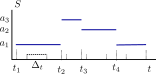
\includegraphics[scale=1.1]{figures/temporal_values.pdf}
\caption{\label{fig:temp} Example of updates for a temporal value of type
 \texttt{Var}.}
\end{center}
\end{figure}

In example depicted in figure \ref{fig:temp}, at current time $t$, the state
of historic of \texttt{Var} $S$ is $[t_1, a_1],[t_2, a_3],[t_3, a_2],[t_4, a_1]$.
Operator \texttt{()} on $S$ will give one of the update value. The signal is 
supposed to be piecewise constant function. Then 
\begin{itemize}
  \item \texttt{S(-0.3)} returns value at time $t - 0.3 * \Delta_t$, ie $a_1$.
  \item \texttt{S(-3.6)} returns value at time $t - 3.6 * \Delta_t$, ie $a_3$.
  \item \texttt{S()} returns last update value, ie $a_1$.
\end{itemize}
Operator \texttt{=} of \texttt{Var} allows to set an update
(for example into the \texttt{compute} function of discrete-time model).

For Vectors (struct \texttt{Vect}):
\begin{itemize}
  \item \texttt{S[1](-0.3)} returns value at time $t - 0.3 * \Delta_t$ for the
  dimension 1.
  \item \texttt{S[0](-3.6)} returns value at time $t - 3.6 * \Delta_t$
  for the dimension 0.
  \item \texttt{S[2]()} returns last update vector at index 2.
  \item \texttt{S[2]=1.5} updates value of $S$ at dim 2 with 1.5.
\end{itemize}

%%%%%%%%%%%%%%%
\subsection{Atomic model interface}
\label{sec:user:atomic}

Evolution of state variables $v_i$ is described by C++ equation syntax close to
mathematical formulation.

For example the expression $V1 = V1(-1) + V2() + V3(-2)$ computes, at current
time $t$, the value of $V1$ as the sum of the value of $V1$ at time 
$t - \Delta_t$, the current value of $V2$ and the value of $V3$ at time 
$t - 2*\Delta_t$. These expressions must be written in the
\texttt{compute} function.

\begin{figure}[!h]
\begin{center} 

\includegraphics[scale=0.80]{figures/userInterface.pdf}
\caption{\label{fig:userInt} A discrete-time model with 6 variables, 3 can be
updated from external event (inputs), 3 are sent by default at each time step 
on the network (outputs).}
\end{center}
\end{figure}

The interface (input and output ports) is given for an example in figure
\ref{fig:userInt}. Note that variables $v_1, \ldots, v_3$ are not necessary
inputs they could also be outputs. And variables $v_4, \ldots, v_6$ could also
have their input ports.

%%%%%%%%%%%%
\subsection{Writing recurrent relations atomic models}
\label{sec:user:diff}

Below is given an example of dynamic for an atomic model that relies 
on the extension {\tt vle.discrete-time}.

\clearpage 

\begin{footnotesize}
\begin{lstlisting}[frame=single, numbers=left] 
class MyModel : public DiscreteTimeDyn
{
public:
  //Declaration of variables
  Var x;
  Vect y;
  Var z; // used in this module as an input
  MyModel(const vd::DynamicsInit& model, 
          const vd::InitEventList& events) :
            DiscreteTimeDyn(model, events)
  {
    //Initialisation of variables from experimental conditions
    x.init(this, "x", events);
    y.init(this, "y", events);
    //Overwrite initialisations (Optionnal)
    x.init_value(3.0);
    x.history_size(3);
    y.dim(2)
  }
  void compute(const vd::Time& /*time*/)
  {
    x =  x(-1) - y[1]() / z();
    y[0] = z() - 1;
    y[1] = y[0]() + 1;
  }
};
\end{lstlisting}
\end{footnotesize}

%%%%%%%%%%%%
\subsection{Configuring atomic models into {\tt vpz} conditions}
\label{sec:user:conf}

The common structure of the conditions for configuring atomic models is the
following:

\begin{itemize}
  \item 'time\_step' (double, default 1.0) : the time step of the discrete time
  atomic model.
  \item 'init\_value\_myvar' (vle::Value, default vle::Double(0.0)) :
  the initial value of the internal variable 'myvar'. It also contains
  the historic values if $history\_size\_myvar > 0$ using e.g.
  vv::Set.
  \item 'dim\_myvar' (int, default 2) : if $myvar$ is a vector, it defines
  the dimension of the vector.
  \item 'history\_size\_myvar' (uint, default 1) : it gives the size of the
  history of internal variable 'myvar'.
  \item 'sync\_myvar' (uint, default 0): if $sync\_myvar > 0$, the value of
  'myvar' at times $n * sync\_myvar * time\_step, \forall n \in \mathbb{N}_+$ is
  expected to be provided by an external event before calling the {\tt compute}
  function.
  \item 'allow\_update\_myvar' (bool, default false): if false, the first
  value set for 'myvar' at a given time step is kept. The following updates for
  'myvar' at this time step are ignored. 
  \item 'error\_no\_sync\_myvar' (bool, default false) : if true, the
  access to 'myvar' at the current time {\tt myvar()} will send an error if the
  last time of update of 'myvar' is before the current time.
  \item 'bags\_to\_eat' (int, default 0) : the number of bags to wait before
  computing the values of variables (calls of {\tt compute} user function).
\end{itemize} 

%%%%%%%%%%%%
\section{Technical details}

%%%%%%%%%%%%
\subsection{Global architecture}
\label{sec:archi}

%\begin{landscape}
%\vspace{-10cm}
\begin{figure}[!h]
\begin{center} 
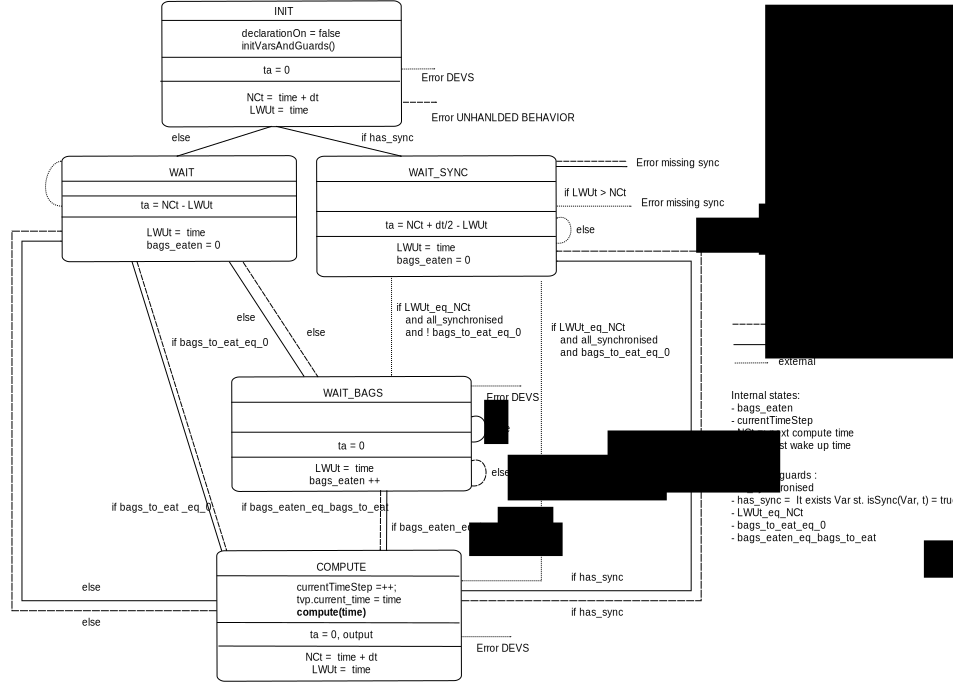
\includegraphics[scale=0.50,angle=0]{figures/DEVS_states.pdf}
\caption{\label{fig:DEVSgraph} The DEVS state transition graph 
for recurrent relations.}
\end{center}
\end{figure}
%\end{landscape}

\subsection{Link to vle.extension.difference-equation}

This package is intended to improve the functionnalities of (package \\
{\tt vle.extension.difference-equation}) and to limit the behavior 
in order to facilitate the coupling with other extensions :
\begin{itemize}
  \item there is no propagation of the perturbation : 
  it requires a state backup and other extensions do not have this.
  \item there is no initialization process of the dynamics (no {\tt initValue}
  function): synchronisation at the time of instantiation of the atomic model
  makes it difficult to couple with DSDEVS. 
  \item There is no external variables. All variables are internal variables. 
  \item It provides vector of variables and polymorphic vle values.
  \item It uses a DEVS state approah for the code of transitions 
  (see fig \ref{fig:DEVSgraph}).
  \item Generalisation and separation of \texttt{DifferenceEquation::Var} 
  into a package \texttt{vle.temporal-values}.
\end{itemize}

Time performances comparison based on 2CV model are given in 
table \ref{table:timeprofiling}. Note that the 2CV-parcelle model
can no be directly translated into discrete-time models since
it uses propagation of perturbation. In order to compare simulation times, 
There is a new version of 2CV-parcelle (2CVdt/2CV-parcelle-de-fusion) where 
CropTT\_TT and CropStade have been merged (propagation of 
perturbation is on CropTT\_TT).  

\begin{figure}
\begin{center}
\begin{tabular}{|c|c|c|c|c|}
\hline
\multirow{2}{*}{model}                        & \multirow{2}{*}{comment} &  \multirow{2}{*}{nb simu} & time (sec)          & time (sec)          \\
~                                             & ~                        &  ~                        & with obs            & without obs         \\\hline\hline
2CV/2CV-parcelle                              & original version         &  200                      & 25                  & 12                  \\ \hline 
\multirow{2}{*}{2CVdt/2CV-parcelle-de-fusion} & merging CropTT           &  \multirow{2}{*}{200}     & \multirow{2}{*}{24} & \multirow{2}{*}{12} \\ 
~                                             & and CropStade            &  ~                        & ~                   & ~                   \\ \hline
\multirow{2}{*}{2CVdt/2CV-parcelle-dt}        & discrete-time            &  \multirow{2}{*}{200}     & \multirow{2}{*}{20} & \multirow{2}{*}{7}  \\ 
~                                             & version                  &  ~                        & ~                   & ~                   \\ \hline
\end{tabular}
\caption{\label{table:timeprofiling}Comparison of time executions given in seconds.}
\end{center}
\end{figure}

\subsection{Source code}

This work has been conducted for vle 1.1.

For vle extensions:
\begin{lstlisting}
git clone https://github.com/rtrepos/packages.git
git checkout -b discreteTime origin/discreteTime
\end{lstlisting}

For 2CV models (discrete time version and original version):
\begin{lstlisting}
git clone http://mulcyber.toulouse.inra.fr/anonscm/git/recordb/recordb.git
git checkout -b discreteTime origin/discreteTime
\end{lstlisting}

%\bibliographystyle{plain}
%\bibliography{biblio}


\end{document}